\section{Debugger}

This section explains how the Overture debugger is constructed. It was build inspired in this \href{http://www.eclipse.org/articles/Article-Debugger/how-to.html}{article}\footnote{\url{http://www.eclipse.org/articles/Article-Debugger/how-to.html}} \cite{Wright&04}.

\begin{figure}[htp]
\centering
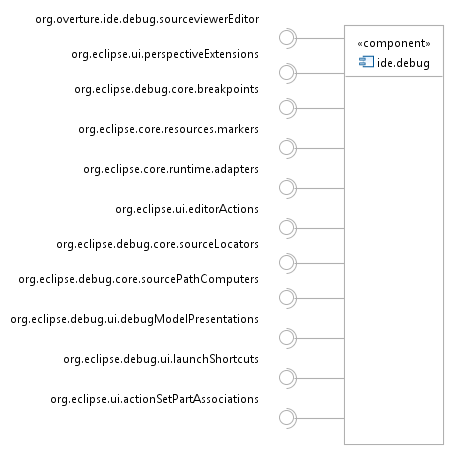
\includegraphics{figures/plugin_ide_debug}
\caption{}
\label{fig:}
\end{figure} 


\subsection{The players}
The debug model defines several entities which should be present in the debug. To incorporate the eclipse debug model we need to implement some classes which are described below:
\begin{description}
\item[IDebugTarget:] is the interface implemented by \class{VdmDebugTraget} and it represents the target in which the model is running, a kind of virtual machine, which can be started and stopped. The class represents the debug environment and it contains the debug threads;

\item[IThread:] implemented by \class{VdmThreads} represents a thread running the model. A thread contains a stackframe;

\item[IStackFrame:] implemented by \class{VdmStackFrame}, it contains information about the call stack and the context variables;

\item[IVariable:] implemented by \class{VdmVariable}, it contains variable values;

\item[IValue:]  implemented by \class{VdmValue}, it contains values or variables. This item and the on above form a treelike structure to represent more complex variables;

\item[IDebugElement:] all of the classes above inherit from this interface. It contains common functions shared by all of them;

\item[IBreakpoint:] implented by \class{VdmBreakpoint} contains information on hwo to break a running model to send to the debugger.
\end{description} 

A visual representation of this relation is shown on figure \ref{fig:debug_model}.
\begin{figure}[htb]
\centering
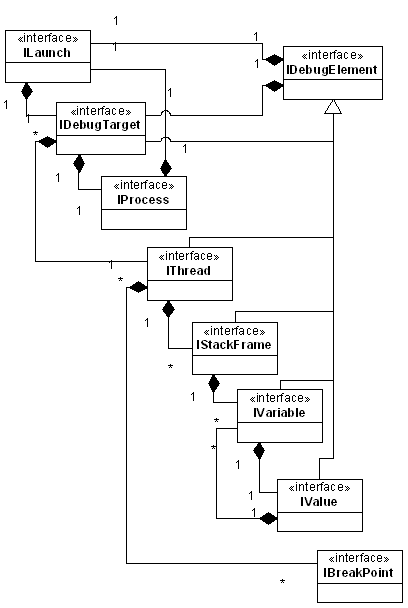
\includegraphics[width=0.8\textwidth]{figures/debug_model}
\caption{Eclipse debug model}
\label{fig:debug_model}
\end{figure}

\subsection{VdmDebugTarget}

This is the class the implements the "virtual machine" where the model to be debugged is running. 

